% background.tex

\documentclass[main.tex]{subfiles}
\begin{document}
\chapter{Background}
\section{Additive Manufacturing}
\emph{Additive Manufacturing} (AM) technologies had their beginnings in the decade of the 1980s. During this time, various independently developed patents were filed across the globe describing a process that would construct an object by selectively adding layers of material -as opposed to removing excess matter or deforming the material to obtain the desired shape. In a way, this represents the core definition of AM: any technology where the final geometry of the manufactured object is obtained through controlled stratification qualifies as an Additive Manufacturing technique \cite{Gibson2015}.

Advancements in the fields of computing, \emph{Computer Aided Design} (CAD), and controllers, among other technological developments, made it possible to quickly translate the patents into working proof-of-concepts, and eventually used as the foundations of commercially successful companies: 1986 saw 3D Systems being founded and in 1989 Scott Crump patented the FDM technology that would give rise to Stratasys \cite{Gibson2015,3DSystems,Stratasys2017}.

\begin{figure}[h]
	\center
	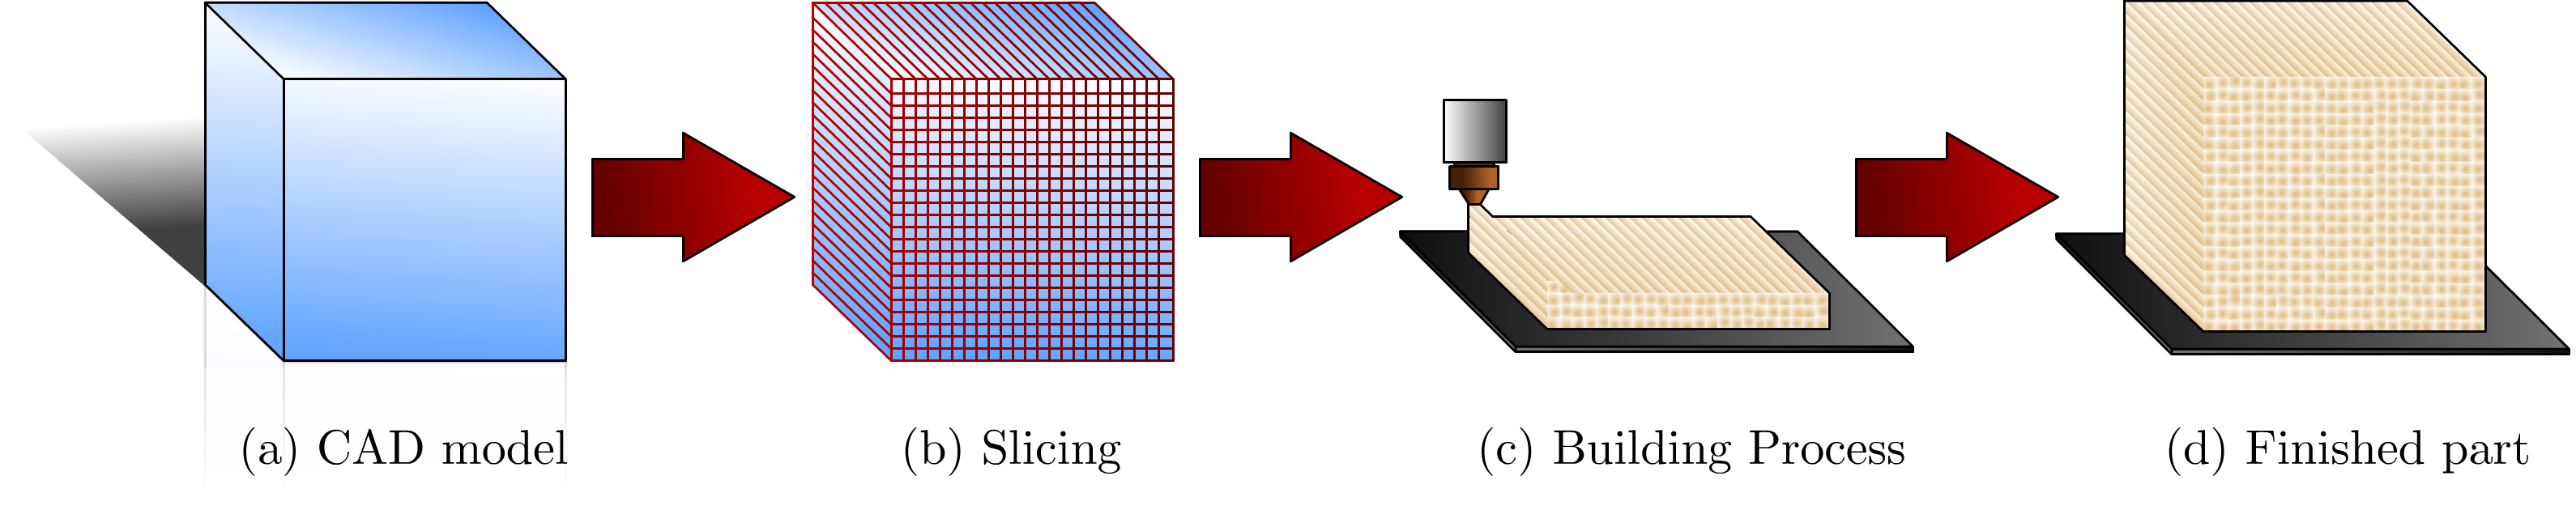
\includegraphics[width=\linewidth]{AM_flowchart_1}
	\caption{Process flow of AM}
\end{figure}
 
\subsection{Fused Filament Fabrication}
%Nomenclature introduced in this chapter:
\nomenclature[A]{SLA}{Stereolithography}% 
\nomenclature[A]{SLS}{Selective Laser Sintering}%
\end{document}